%!TEX root = SysSpec_ClockPendulumAnalyzer.tex
\subsection{Sequenzdiagramm}
In diesem Kapitel werden einzelne Arbeitsabläufe anhand eines Sequenzdiagrammes dargestellt.
	\subsubsection{Start und Speichern einer Datenmessung}
    Dieses Sequenzdiagramm (Abbildung \ref{fig:sequence_save}) zeigt den Ablauf der Hauptfunktionalität.
    Zuerst werden alle zusätzlich benötigten Teilnehmer gestartet.
    Danach beginnt der Speichervorgang einzelner Datenmessungen.
    Dabei ruft das Programm die FIFO\footnote{First In, First Out}-Liste ab, welche durch die UART Kommunikation mit Messwerten befüllt wird.
    Sind 5 Datentupel aus der FIFO Liste gelesen, werden diese in der Datenbank gespeichert.
    \begin{figure}[H]
        \centering
        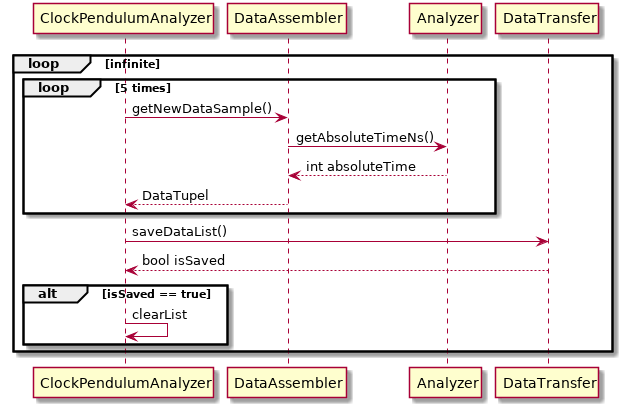
\includegraphics[width=\textwidth]{sequence_data_save.png}
        \caption{Sequenzdiagramm zum Speichern der Daten}
        \label{fig:sequence_save}
    \end{figure}

    \clearpage
    \subsubsection{Abrufen einer Datenmessung}
    Ein Webclient ruft Daten über eine HTTP Request auf die angebotene REST Schnittstelle.
    Als Antwort erhält er eine JSON Struktur der Messdaten.
    Das ganze wird im Sequenzdiagramm (Abbildiung \ref{fig:sequence_get}) unten abgebildet (mit dem Uhrennamen-Parameter als Beispiel).
    \begin{figure}[H]
        \centering
        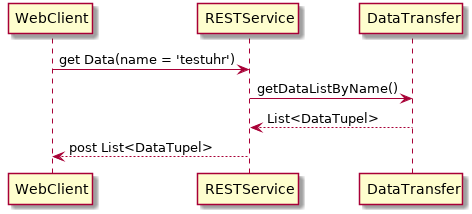
\includegraphics[width=.7\textwidth]{sequence_data_access.png}
        \caption{Sequenzdiagramm zum Aufrufen der Daten}
        \label{fig:sequence_get}
    \end{figure}